\chapter{Cadenas de caracteres}

\section{Invertir una cadena de texto}

\textit{Escriba un programa que le permita invertir una palabra ingresada, por ejemplo, si usted 
introduce MATLAB deberá devolverle BALTAM.}

\sol

En esencia lo que se debe hacer es \textit{invertir} los indices del vector tipo char en 
el cual se guarda la cadena de texto.

\begin{verbatim}
cad=input('Introduzca una palabra: ','s');
disp(cad((end:-1:1)));
\end{verbatim}

\section{Contar palabras}

\textit{Desarrolle un script que reciba como entrada una cadena de caracteres y que devuelva 
la cantidad de palabras que la componen. Para este caso se asumirá que el texto pasado como dato 
de entrada tiene una estructura coherente y libre de cualquier secuencia extraña de signos de 
puntuación u otro tipo de caracteres diferentes a los alfanuméricos.}

\sol

\begin{verbatim}
txt = input('Inserte un texto: ','s');
resto = txt;
k = 0; % Inicializa contador
while true
   [palabra, resto] = strtok(resto, ' ');
   if isempty(palabra),  break;  end
   k = k + 1;
end
fprintf('No. de palabras encontradas: %d\n\n',k);
\end{verbatim}


\section{Contar vocales en una cadena de texto}

\textit{Escriba un programa que reciba como entrada una frase o cadena de texto y que muestre como salida el número de vocales que contiene dicha frase.}

\sol

\begin{verbatim}
cad=input('Introduzca una cadena de texto: ','s');
k=0;
for i=1:length(cad)
    switch cad(i)
        case {'A','a','E','e','I','i','O','o','U','u'}
            k=k+1;
        otherwise
            % ...
    end
end
fprintf('Numero de vocales: %g\n\n',k);
\end{verbatim}


\section{Ordenar palabras}

\textit{Escriba un programa que ordene las palabras contenidas en una cadena de caracteres, imprimiéndolas en pantalla.}

\sol



\section{Cifrado básico}

\textit{El método de cifrado más simple es el cifrado por desplazamiento, que consiste en remplazar un caracter 
por otro ubicado {\bf n} posiciones a la derecha en la tabla de código ASCII. Por ejemplo, si tenemos la palabra 
{\bf perro}, y queremos cifrarla desplazando tres lugares obtendríamos: {\bf shuur}. En la figura siguiente se muestra 
un esquema de lo anterior.}

\begin{center}
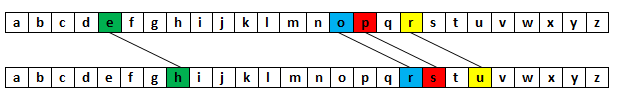
\includegraphics[scale=0.8]{src/cifrado.png}
\end{center}

\textit{Desarrolle un programa que tenga como entrada una cadena de caracteres y devuelva en pantalla 
la cadena cifrada mediante el desplazamiento por tres posiciones.}


